\documentclass[main.tex]{subfiles} 
\begin{document}

\section*{Drøfting}

\subsection*{Høyt presterende og evnerike elever}

I opplæringsloven \S 1-3 angis det at opplæringen skal tilpasses til den enkelt elevs ``evner og forutsetninger''.  Elever med stort læringspotensial er også en elevgruppe som må ivaretas i klasserommet. Dette er elever som viser faglig sammenhenger, er reflekterte og har god formuleringsevne. Fra lærerens perspektiv er det ofte ikke nødvendig med motivasjonsarbeid, derimot kan slike elever kjede seg hvis de ikke blir faglig utfordret (\citeNP{brgu16}). Disse elever har nytte av tilbakemeldinger som hjelper de med å jobbe målrettet. Videre må det eksistere en aksept for å være flink i klasserommet, dette skaper trygghet. Et slikt aksept blir oppfostret gjennom god klassemiljø og gjennom lærers egen oppmerksomhet til slike elever. Høyt presterende elever har også gode rutiner med å være forberedt til undervisningssekvenser, her kan jeg som lærer bruke deres forkunnskaper til å engasjere disse elevene i en dialog. Til slutt ligger det innenfor lærerens profesjonsetisk ansvar å ivareta slike elever fra presset med å alltid være best (\citeNP{brev17}). 
\newline\newline
Jeg kan tilpasse opplæringen ved å tilby høyt presterende elever nivå-delte oppgaver og oppgaver som er kognitiv utfordrende. I slike tilfeller kan rike åpne oppgaver brukes til å la slike elever ha muligheten til å gå dypere i fagstoff og trekke faglig sammenhenger.  Derfor er det viktig å være bevisst på hvor mange frihetsgrader elever skal få (\citeNP[s. 29]{knai11}). Jo flere beslutninger eleven må ta selv, jo åpnere er oppgaven.
\newline\newline 
I denne diskursen har jeg snakket kortfattet om høyt presterende elever. I litteraturen skilles det mellom høyt presterende elever og evnerike elever (\citeNP{brgu16}; \citeNP[s. 208]{kolb14}). Også denne elevgruppen har behov for tilpasset opplæring. Manglende tilpasset opplæring kan medføre en negativ holdning til skolen generelt, og til læring i skoleregi spesielt (\citeNP[s. 208]{kolb14}). Her kan mulige tiltak være bruk av både organisatorisk differensiering og pedagogisk differensiering. Til vanlig skal ikke organisatorisk differensiering brukes som et fast virkemiddel, men forskning viser at slike elever har behov for å tilbringe tid med andre på samme intellektuell nivå (\citeNP[s. 215]{kolb14}). Gjennom pedagogisk differensiert undervisning kan tiltak som tempo brukes til å forsere eleven i pensum, fag og trinn. Et slikt tiltak tillater at eleven forblir en del av mangfoldet og prinsippet om tilpasset opplæring ivaretas.


\subsection*{Elever med minoritetsspråklig bakgrunn og svakt presterende elever}

Manglende opplevd støtte i relasjonen til læreren på videregående skole er en klar risikofaktor for svakere skoleresultater og redusert motivasjon for elever med innvandringsbakgrunn (\citeNP[s. 70]{hegn13}). Videre er den praktiske oppfølgingen av hjemmearbeid og leksehjelp er ikke like sterk når elevene når lengere opp i utdanningsløpet (\citeNP[s. 69]{hegn13}). 
\newline\newline
Her kan jeg som lærer på ungdomstrinn stille tydelig krav og forventninger fra elevene, bruke formativ vurdering underveis til å følge opp enkelt elever helt fra starten og jobbe målrettet mot både kortsiktige og langsiktige mål som jeg og eleven setter sammen. Ifølge \citeA{brbl14} skal jakt etter bevis på læring kunne brukes aktivt av læreren og elevene for å avgjøre hvor de er i sin læring, hva de bør jobbe videre med, og hvordan de kan gå fram for å få det til (\citeNP[s. 1]{brbl14}). Sist men ikke minst kan jeg bidra til å opprettholde gode relasjoner med eleven og jobbe med å skape en god klassemiljø. Gjennom naturfagstimen kan jeg tilpasse opplæringen ved å bruke elevenes bakgrunn, nivå og tempo.
\newline\newline
Tilslutt kan det være elever som har rett til spesialundervisning etter en sakkyndig vurdering av PP-tjenesten. Disse elevene vil da jobbe med andre læringsmål enn hva resten av klassen jobber med. Her ligger det innenfor mitt profesjonelle ansvar å følge opp disse elevene etter en utarbeidet individuell opplæringsplan (\citeNP{udirSU}).


\subsection*{Representasjoner}

Til denne oppgaven har jeg valgt å fokusere på kompetansemål relatert til organisk kjemi. Ofte når elever blir introdusert til organisk kjemi er deres første stoppested ved hydrokarboner og navnsetting av hydrokarboner. Gjennom egen praksiserfaring har jeg opplevd dette som en fin introduksjon til det overordnede temaet organisk kjemi. Mange elever opplever initielt vansker med navnsetting av blant annet hydrokarboner, mens noen elever opplever innføringen systematisk og klarer fort å beherske navnsetting og beveger seg videre til andre temaer som alkoholer, karboksylsyrer og karbohydrater. Progresjon til disse temaene har en naturlig overgang, fra å lære seg å navnsette hydrokarboner til å utvide de kjemiske forbindelsene ved å legge til hydroksylgrupper og karboksylgrupper. \newline

\begin{figure}[h!]
\centering
    \begin{subfigure}{.5\textwidth}
    \centering
    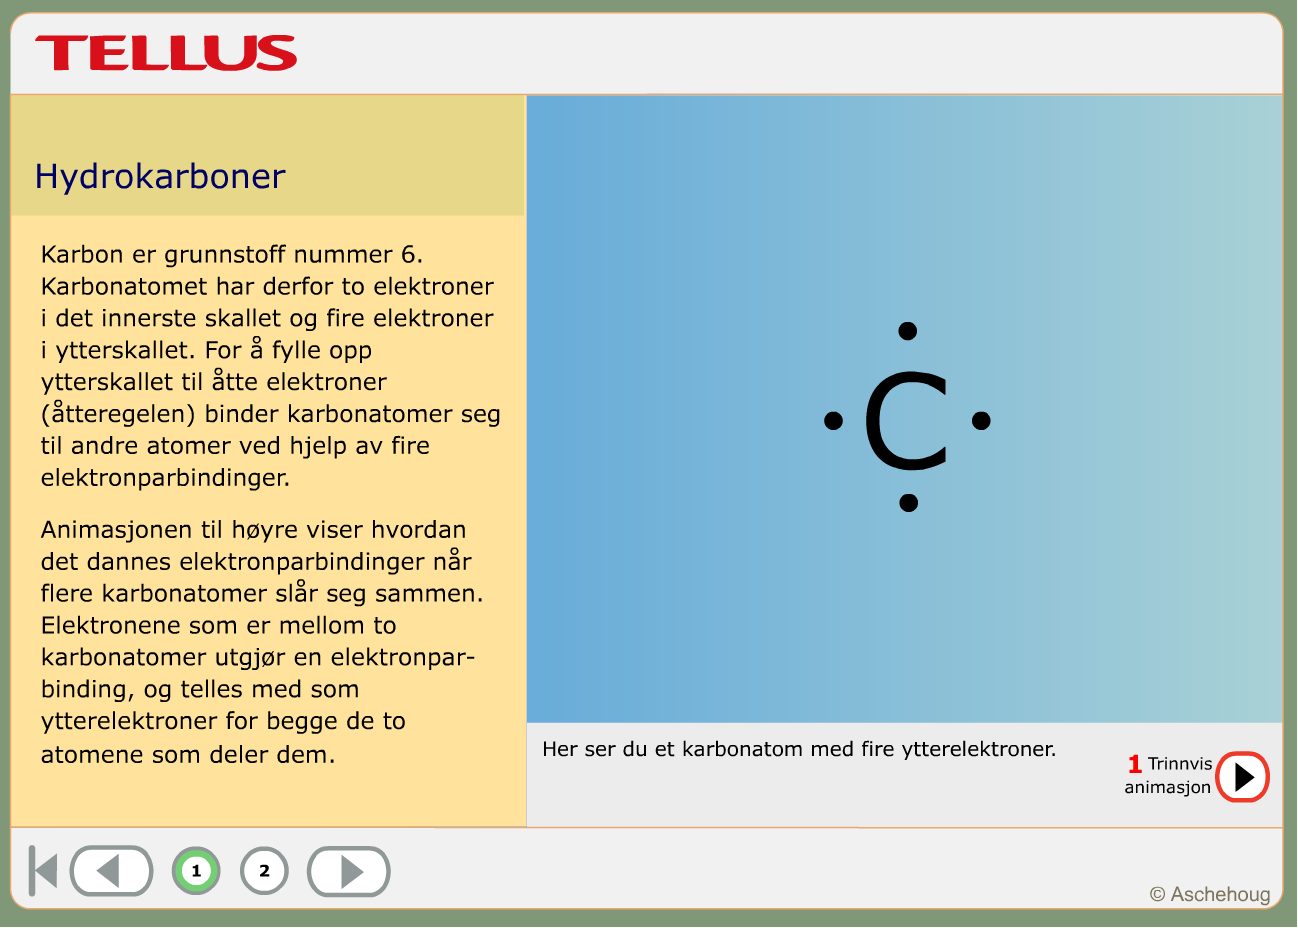
\includegraphics[scale = 0.20]{../figures/lokus1.png}
    \end{subfigure}%%
    \begin{subfigure}{.5\textwidth}
    \centering
    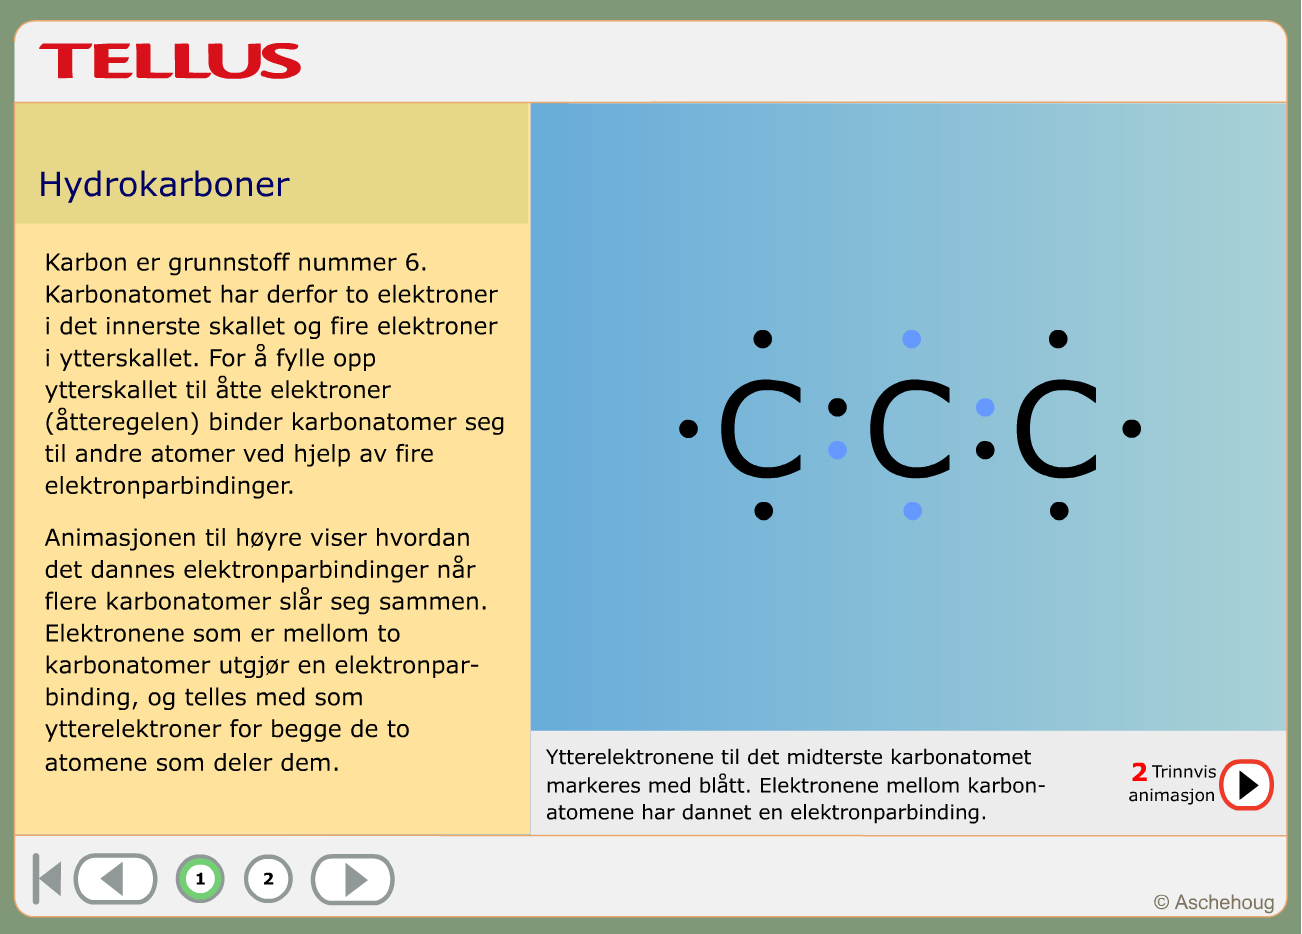
\includegraphics[scale = 0.199]{../figures/lokus2.png}
    \end{subfigure}
    \begin{subfigure}{.5\textwidth}
    \centering
    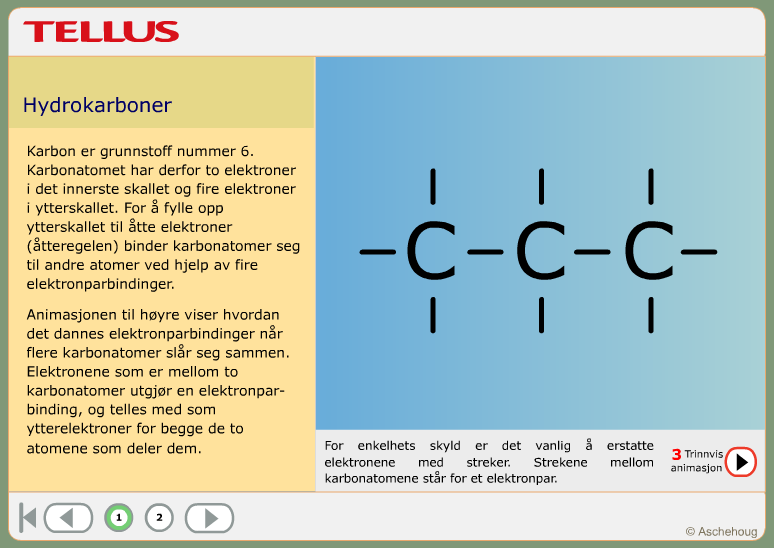
\includegraphics[scale = 0.34]{../figures/lokus3.png}
    \end{subfigure}%%
    \begin{subfigure}{.5\textwidth}
    \centering
    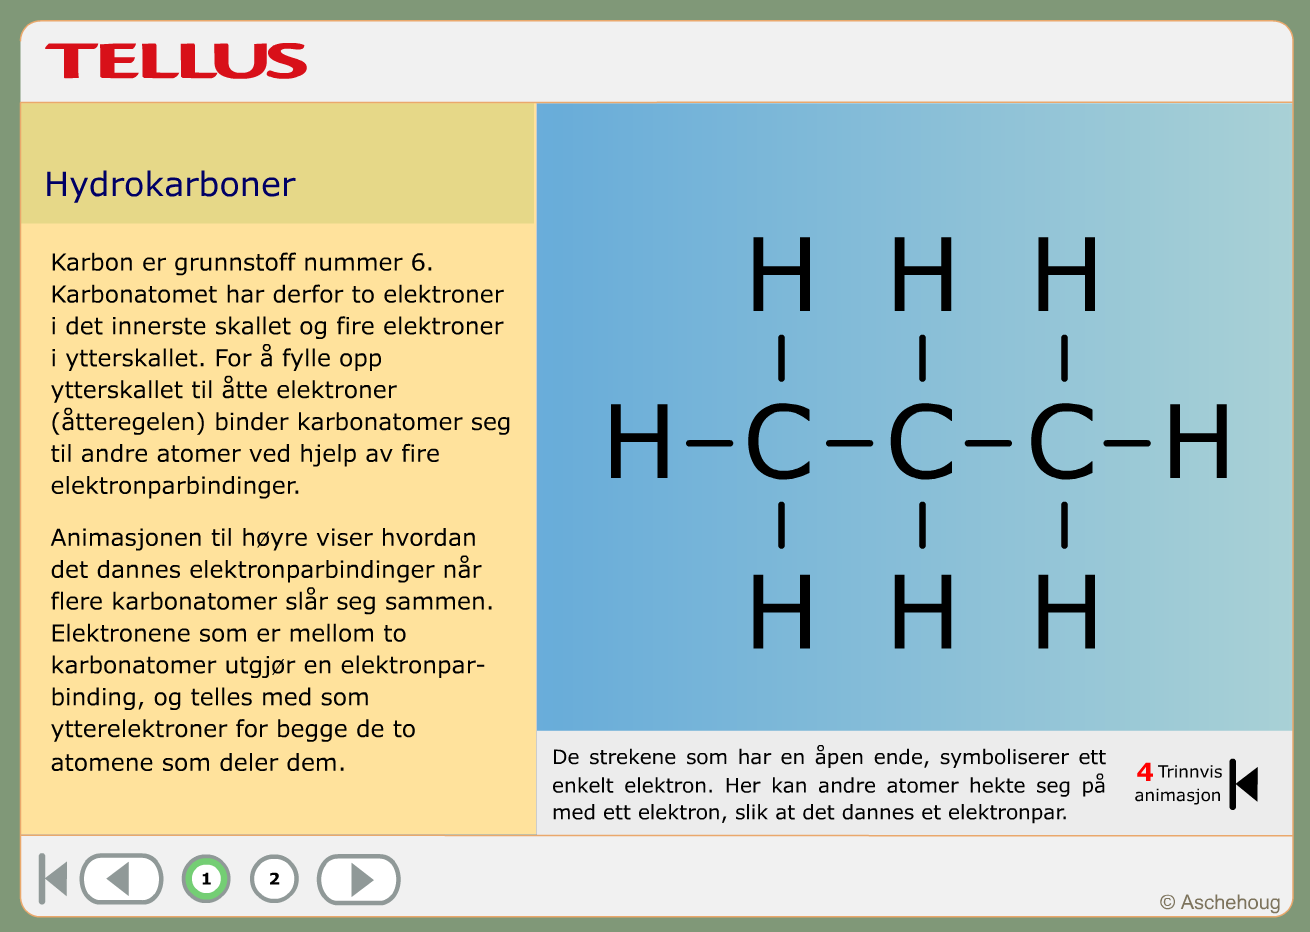
\includegraphics[scale = 0.199]{../figures/lokus4.png}
    \end{subfigure}
    \caption{Interaktiv forklaring for elektronparbindinger når flere karbonatomer slår seg sammen. Kilde: 
    \protect\url{http://www3.lokus.no/flashEmbedder.jsp?contentItemId=52275952&selectedLanguageId=1&title=hydrokarboner}}
    \label{fig:lokus}
\end{figure}

\hspace{-6mm}Her kan vi se at elevene må ha en god begrepsforståelse for at de skal kunne danne en fagovergripelig forståelse. Mork og Erlien skriver at begreper er kanskje det området i naturfag som forårsaker flest problemer for læring, fordi noen begreper kan være veldig abstrakte (\citeNP[s. 24]{moer10}). Elever som har vansker med å navnsette og skille hydrokarboner, alkoholer og organiske syrer, har også ofte problemer med å visualisere de kjemiske forbindelsene, eller tolke strukturformelen. Det blir enda vanskeligere for disse elevene når begreper alkaner, alkener og alkyner innføres, det vil si enkelt, dobbelt og trippelbindinger. Da må de i tillegg holde oversikt over bindinger og hvor hydrogenatomer kan forbinde seg til karbon-atomet. Derfor er det viktig for både de lavt presterende -og høyt presterende elevene at de kan ha gode illustrasjoner som kan visualisere teorien på en forståelig vis. Dersom målet med undervisningen er at alle elever skal forstå det som undervises er det da viktig å treffe hver enkelt elev som har ulik tilnærming til stoff og gi hver elev mange erfaringer innenfor samme tema (\citeNP[s. 32]{froy10}). \newline

\begin{figure}[h!]
\centering
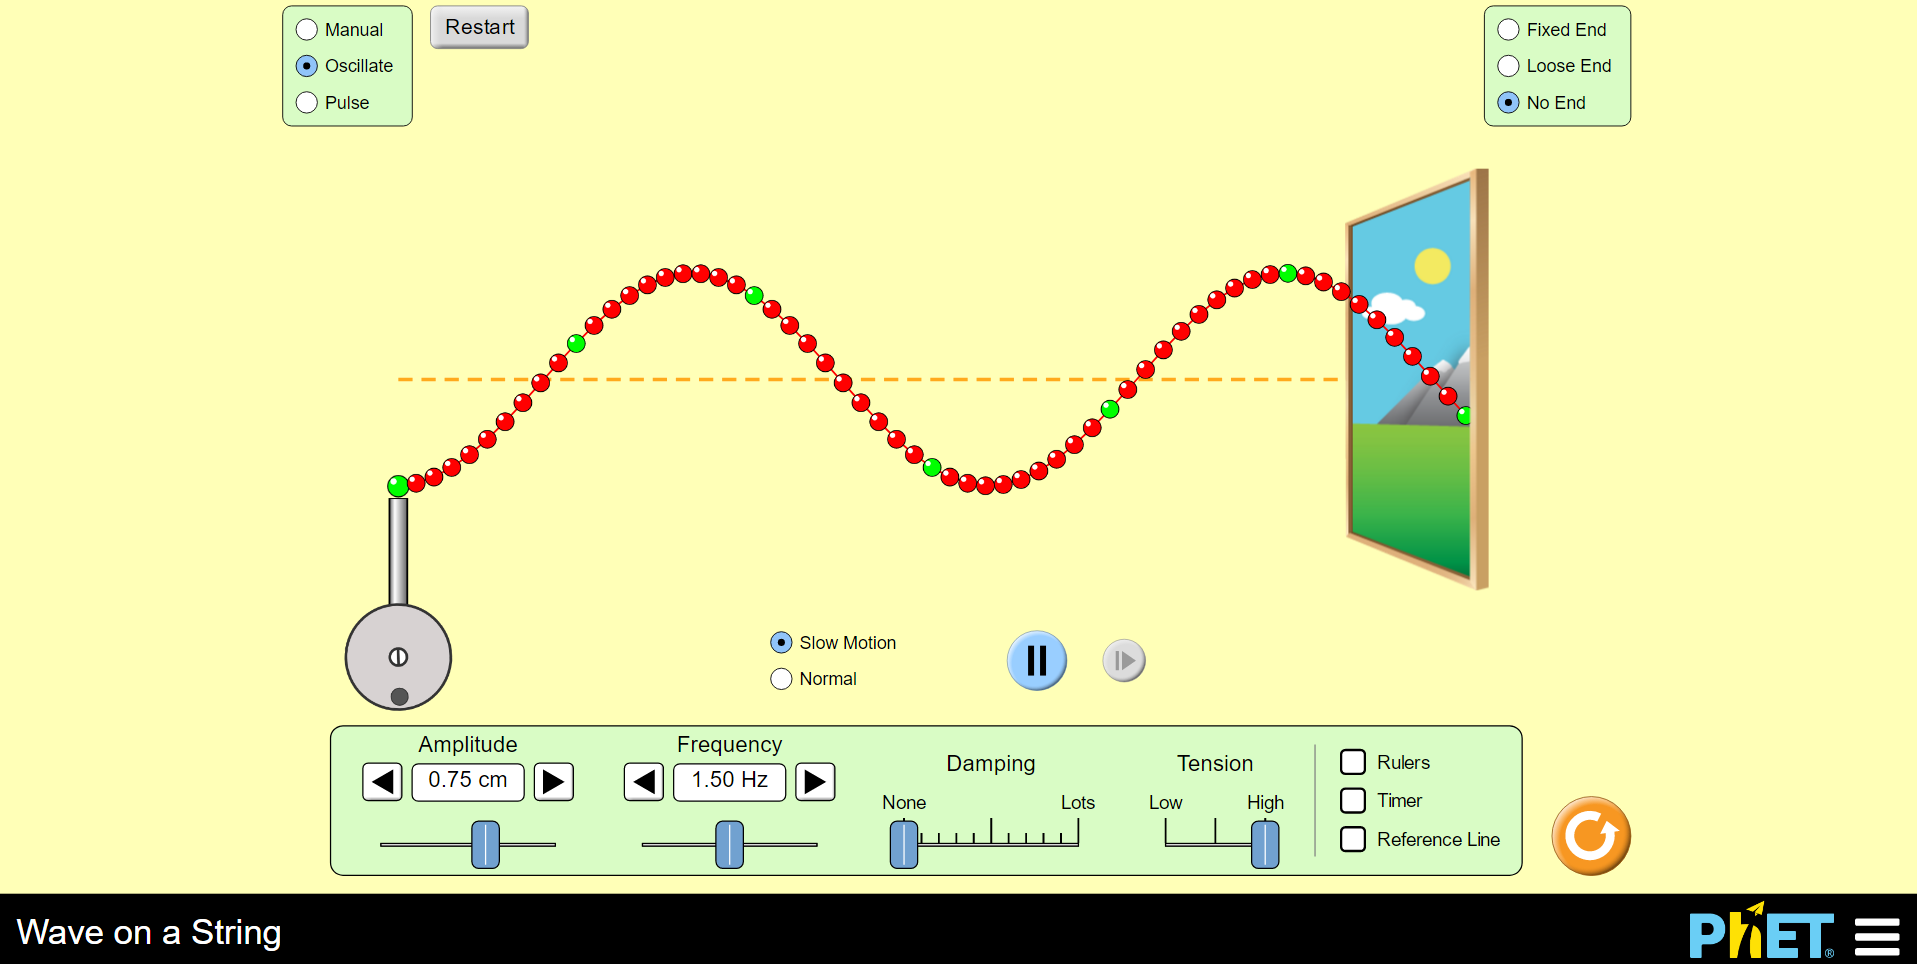
\includegraphics[scale = 0.25]{../figures/wave.png}
\caption{Interaktiv simulering av en oscillerende streng. Kilde: 
\protect\url{https://phet.colorado.edu/sims/html/wave-on-a-string/latest/wave-on-a-string_en.html}}
\label{fig:wave}
\end{figure}

\hspace{-6mm}Bruk av interaktive programer (f.eks flash basert nettside Lokus - se figur \ref{fig:lokus}) kan ha en gunstig virkning og hjelpe de lavt presterende elevene med å skape motivasjon. Et annet virkemiddel er et molekylbyggesett. Her kan elevene få en fysisk tilknytning til strukturene de leser om og navnsetter gjennom førstehåndserfaring (\citeNP[s. 111]{froy10}). Gjennom min egen praksiserfaring har jeg opplevd at bruk av molekylbyggesett kan være motiverende og innlysende. Når elever forsøker å lage fysiske bindinger mellom karbonatomer og andre atomer ser mange at det er begrenset hvordan disse bindingene kan skapes. Derfor har slike byggesett en didaktisk betydning for elevene. \newline

\begin{figure}[h!]
\centering
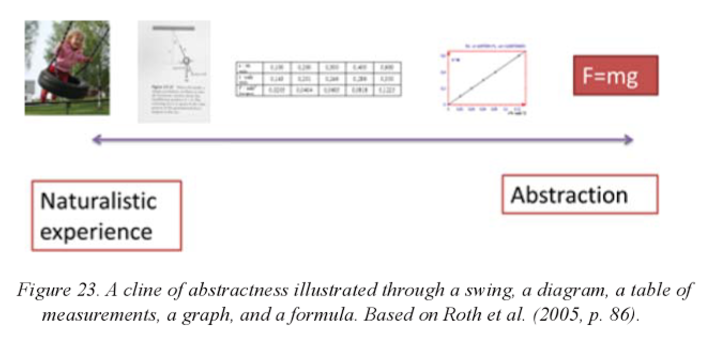
\includegraphics[scale = 0.6]{../figures/knain.png}
\caption{Grad av abstraksjoner. Kilde: \protect\citeA[s.80]{knai15}}
\label{fig:knain}
\end{figure}

\newpage
%%%%%%%%%%%%%%%%%%%%%%%%%%%%%%%%%%%%%%%%%%%%%%%%%%%
\hspace{-6mm}I denne oppgaven er fokuset rundt tekster og illustrasjoner for å skape en tilpasset opplæring. Her har jeg snakket om en spesifikk naturfagstime som hovedsakelig dreier seg om innføring av hydrokarboner og navnsetting av hydrokarboner ved hjelp av strukturformel. Gjennom andre temaer jeg har undervist jeg har erfart at bruk av simuleringer (f.eks nettside PhET Interactive Simulations : se figur \ref{fig:wave}) kan også skape variasjon og motivasjon blant elever på tvers av faglig nivå. Jeg brukte simuleringen i figur \ref{fig:wave} til å koble temaet elektromagnetisk stråling til frekvens og bølgelengde av en oscillerende streng. Det viste seg at elever som ellers ikke er aktive i timen viste stor intresse og forsøkte å få simuleringen til å virke autentisk ved å endre på parametere.\
\newline\newline
\citeA[s. 80 - 81]{knai15} skriver at slike representasjoner binder tekst og illustrasjoner fra bøker til en direkte erfaring eller video som viser. Han illustrer dette (se figur \ref{fig:knain}) ved å sette direkte erfaring på en side av abstraksjonsskalaen til ren abstraksjoner (som f.eks formler) på den andre siden. Fra lærerens side kreves det god faglig kompetanse for å finne ut om en simulering eller animasjon fremstiller en naturfaglig prosess riktig. 

\newpage
%%%%%%%%%%%%%%%%%%%%%%%%%%%%%%%%%%%%%%%%%%%%%%%%%%%
\hspace{-6mm}En faglig dyktig lærer ser ofte mange muligheter og er kreativ når det gjelder valg av metoder og tilrettelegging (\citeNP[s. 148]{moer10}). For eleven innebærer valg av gode representasjoner økt evne til å lese en tekst eller lærebok (\citeNP[s. 84]{knai15}).


\end{document}